\documentclass[tikz,border=3mm]{standalone}
\usepackage{pgfplots}
\pgfplotsset{compat=newest}
\pgfplotsset{
    colormap={bluered}{
    rgb255(0cm)=(0,0,180); rgb255(1cm)=(0,255,255); rgb255(2cm)=(100,255,0);
    rgb255(3cm)=(255,255,0); rgb255(4cm)=(255,0,0); rgb255(5cm)=(128,0,0)}
}

\begin{document}

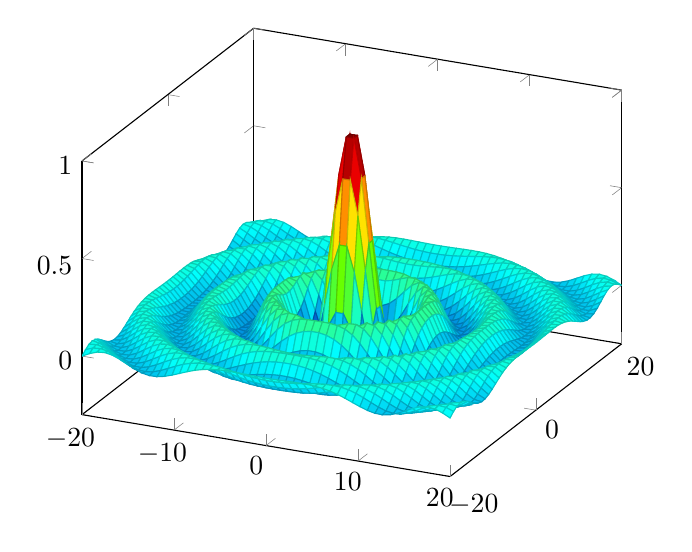
\begin{tikzpicture}
    \begin{axis}
    [
        domain=-20:20,
        xmin=-20, xmax=20,
        ymin=-20, ymax=20,
        zmin=-.3, zmax=1,
        samples=50,
        % axis y line=center,
        % axis x line=center,
        % axis z line=middle
    ]
        \addplot3[surf,]{sin(sqrt(x^2 + y^2)*(180/pi))/sqrt(x^2+y^2)};
    \end{axis}
\end{tikzpicture}

\end{document}
